% !TEX encoding = UTF-8 Unicode
% !TEX root = DesignDocument.tex

\section{Website}
\subsection{Considerations}

\tab The following sections will cover detailed instructions for publication and deployment of a C\# ASP.NET web application. The publication and deployment steps themselves are relatively simple but there are other factors of the project design that must be taken into consideration before publishing.  

\begin{enumerate}
    \item \textbf{Hosting Environment}\\

    \tab While ASP.NET Framework web applications are still only supported for production deployments on Windows IIS and Kestrel servers, ASP.NET Core 2+ web applications have been sourced to allow cross-platform production deployment. For this reason, the Visual Studio IDE provides several options for publication targets. These options include:

    \begin{itemize}
        \item Microsoft Azure Virtual Machines
        \item Microsoft Azure App Service -- This is the publication target that will be covered.\\
        
        \tab The Microsoft Azure related publication targets are for web applications that will run within the Azure hosted services suite. These methods of publication will directly write all new web application source code files to the associated execution directory within the Azure service.  Assuming successful publication, deployment is automatic.\\
        
        \item IIS, FTP\\
        
        \tab The IIS, FTP publication target is for directly deploying to the inetpub directory of a Windows Server that the web application developer has credentials and permissions to.  This is similar to the Azure publication target procedure except to a non-Azure Windows Server machine.\\
        
        \item Folder\\
        
        \tab The folder publication target is for writing all new web application source code to a local directory on the development machine. This allows more flexibility for custom web application publications.
    \end{itemize}
\end{enumerate}

\subsection{Publication}

\tab The following are steps for web application publication to a Microsoft Azure App Service.

\begin{figure}[H] 
    \centering
    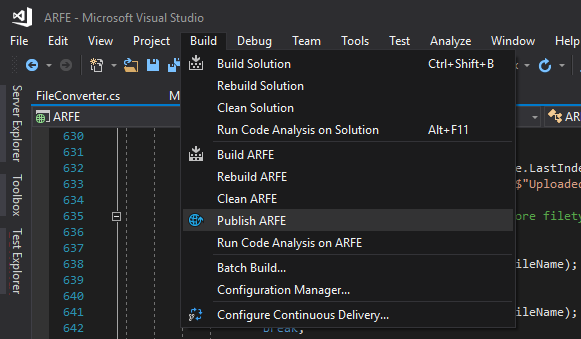
\includegraphics[scale=.5]{select_publish}
\end{figure}
    \begin{figure}[H] 
        \centering
        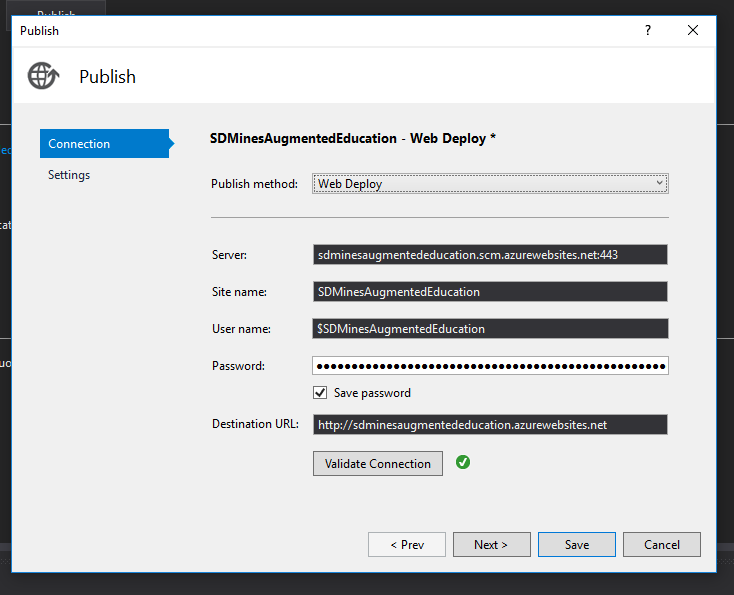
\includegraphics[scale=.5]{connection}
    \end{figure}

    
    
    \begin{figure}[H] 
        \centering
        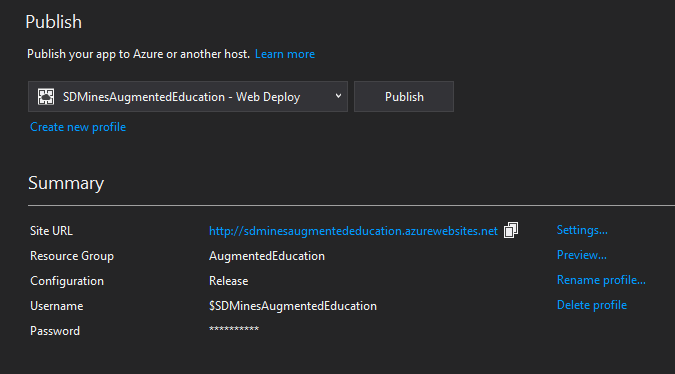
\includegraphics[scale=.5]{review_settings}
    \end{figure}
    
    \begin{figure}[H] 
        \centering
        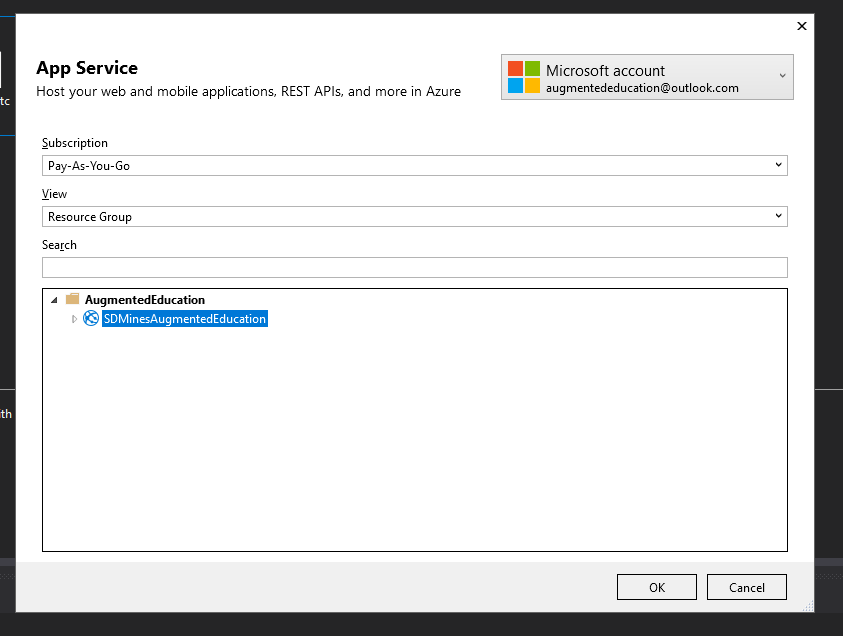
\includegraphics[scale=.5]{select_app_service}
    \end{figure}
    
    \begin{figure}[H] 
        \centering
        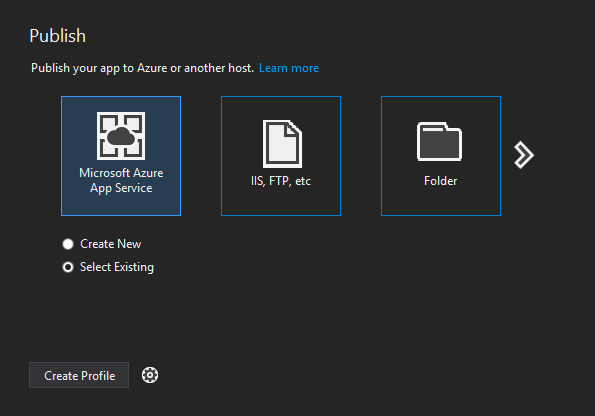
\includegraphics[scale=.5]{select_existing}
    \end{figure}
    
    
    \begin{figure}[H] 
        \centering
        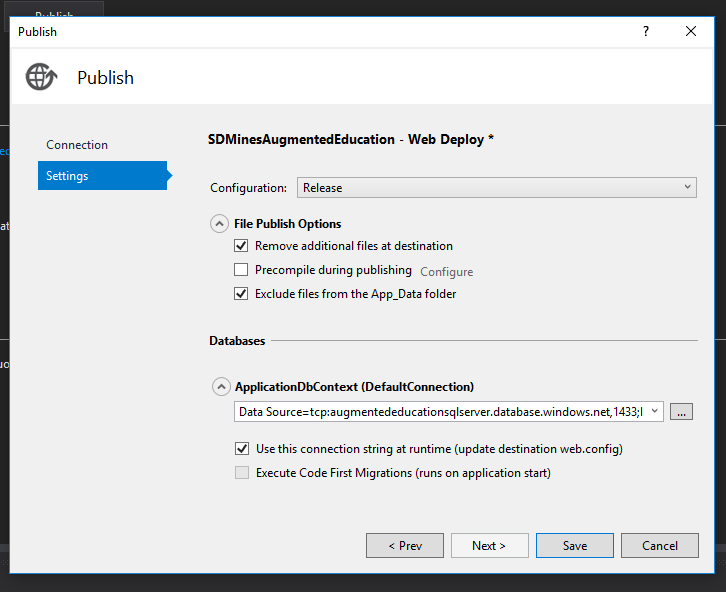
\includegraphics[scale=.5]{settings}
    \end{figure}
    
    
    
    
    
    
    
    
    \begin{figure}[H] 
        \centering
        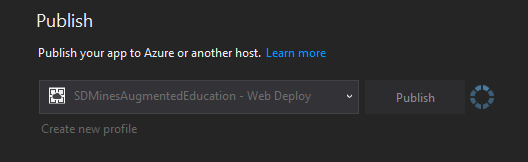
\includegraphics[scale=.5]{publish}
    \end{figure}
    
    \begin{figure}[H] 
        \centering
        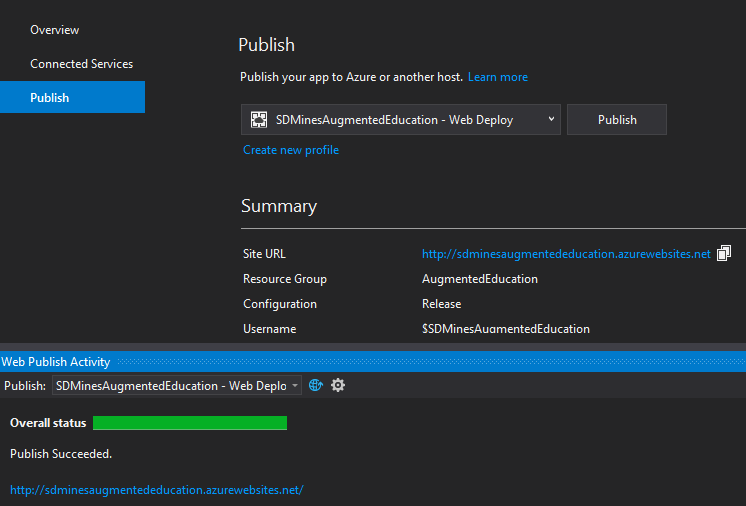
\includegraphics[scale=.5]{publish_succeeded}
    \end{figure}
    
    
\subsection{Deployment}